% This file was created by tikzplotlib v0.9.8.
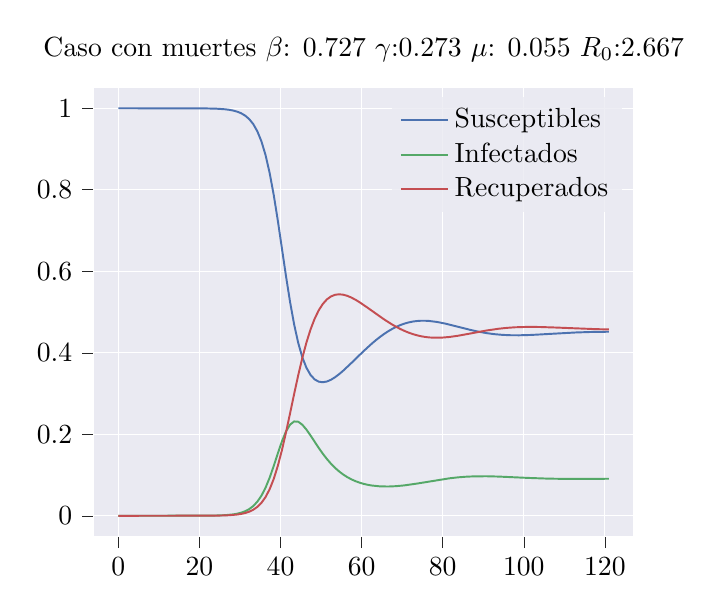
\begin{tikzpicture}

\definecolor{color0}{rgb}{0.917647058823529,0.917647058823529,0.949019607843137}
\definecolor{color1}{rgb}{0.298039215686275,0.447058823529412,0.690196078431373}
\definecolor{color2}{rgb}{0.333333333333333,0.658823529411765,0.407843137254902}
\definecolor{color3}{rgb}{0.768627450980392,0.305882352941176,0.32156862745098}

\begin{axis}[
axis background/.style={fill=color0},
axis line style={white},
legend cell align={left},
legend style={fill opacity=0.8, draw opacity=1, text opacity=1, draw=none, fill=color0},
tick align=outside,
tick pos=left,
title={Caso con muertes
\(\displaystyle \beta\): 0.727 \(\displaystyle \gamma\):0.273 \(\displaystyle \mu\): 0.055 \(\displaystyle R_0\):2.667},
x grid style={white},
xmajorgrids,
xmin=-6.05, xmax=127.05,
xtick style={color=white!15!black},
y grid style={white},
ymajorgrids,
ymin=-0.0499999978586724, ymax=1.04999995503212,
ytick style={color=white!15!black}
]
\addplot [line width=0.7pt, color1]
table {%
0 1
21.1749992370605 0.999672889709473
24.2000007629395 0.998904466629028
26.216667175293 0.997550010681152
27.2250003814697 0.996339321136475
28.2333335876465 0.994535326957703
29.2416667938232 0.99185311794281
30.25 0.987878441810608
31.2583332061768 0.982017517089844
32.2666664123535 0.973437428474426
33.2750015258789 0.961008429527283
34.283332824707 0.943276047706604
35.2916679382324 0.918517351150513
36.2999992370605 0.884965062141418
37.3083343505859 0.841278910636902
38.3166656494141 0.787242412567139
39.3250007629395 0.724441170692444
41.341667175293 0.588185787200928
42.3499984741211 0.524545431137085
43.3583335876465 0.469174027442932
44.3666648864746 0.423887252807617
45.375 0.388871908187866
46.3833351135254 0.36326265335083
47.3916664123535 0.345714092254639
48.4000015258789 0.334791421890259
49.408332824707 0.329174757003784
50.4166679382324 0.327734589576721
51.4249992370605 0.329540014266968
52.4333343505859 0.333836317062378
53.4416656494141 0.340015411376953
54.4500007629395 0.347586035728455
55.4583320617676 0.356150150299072
57.4749984741211 0.375014781951904
60.5 0.404276013374329
62.5166664123535 0.422583937644958
63.5250015258789 0.43104612827301
64.533332824707 0.438940286636353
65.5416641235352 0.446203708648682
66.5500030517578 0.452785968780518
67.5583343505859 0.458648562431335
68.5666656494141 0.463764309883118
69.5749969482422 0.468116760253906
70.5833358764648 0.471700429916382
71.591667175293 0.474521160125732
72.5999984741211 0.476595282554626
73.6083297729492 0.477949857711792
74.6166687011719 0.478622555732727
75.625 0.478660583496094
76.6333312988281 0.478120088577271
78.6500015258789 0.475564002990723
80.6666641235352 0.471525549888611
83.6916656494141 0.464010238647461
86.716667175293 0.456392526626587
88.7333297729492 0.451960802078247
90.75 0.448349714279175
92.7666702270508 0.445674180984497
94.783332824707 0.443940281867981
96.8000030517578 0.443073034286499
98.8166656494141 0.442943334579468
101.841667175293 0.443783640861511
106.883331298828 0.446601152420044
112.933334350586 0.449896335601807
116.966667175293 0.451185464859009
121 0.45164167881012
};
\addlegendentry{Susceptibles}
\addplot [line width=0.7pt, color2]
table {%
0 0
23.1916675567627 0.000457644462585449
26.216667175293 0.00153017044067383
28.2333335876465 0.003409743309021
29.2416667938232 0.00507891178131104
30.25 0.00754702091217041
31.2583332061768 0.0111745595932007
32.2666664123535 0.0164593458175659
33.2750015258789 0.0240594148635864
34.283332824707 0.034785270690918
35.2916679382324 0.0495208501815796
36.2999992370605 0.0690141916275024
37.3083343505859 0.0935003757476807
38.3166656494141 0.122211217880249
39.3250007629395 0.153014540672302
40.3333320617676 0.18256139755249
41.341667175293 0.207133054733276
42.3499984741211 0.223854303359985
43.3583335876465 0.231556177139282
44.3666648864746 0.230830669403076
45.375 0.223436951637268
46.3833351135254 0.211540579795837
47.3916664123535 0.197150588035583
49.408332824707 0.166729331016541
50.4166679382324 0.152483105659485
51.4249992370605 0.139479994773865
52.4333343505859 0.127876877784729
53.4416656494141 0.117694020271301
54.4500007629395 0.108872532844543
55.4583320617676 0.101312041282654
56.466667175293 0.0948954820632935
57.4749984741211 0.0895036458969116
58.4833335876465 0.0850231647491455
59.4916648864746 0.0813509225845337
60.5 0.0783951282501221
61.5083351135254 0.0760753154754639
62.5166664123535 0.074321985244751
64.533332824707 0.0722805261611938
66.5500030517578 0.0718734264373779
68.5666656494141 0.0727839469909668
70.5833358764648 0.0747363567352295
73.6083297729492 0.0790376663208008
81.6750030517578 0.0920324325561523
83.6916656494141 0.0943088531494141
85.7083358764648 0.0959087610244751
87.7249984741211 0.0968241691589355
90.75 0.0970619916915894
93.7750015258789 0.0962967872619629
100.833335876465 0.0930855274200439
105.875 0.0912716388702393
110.916664123535 0.0904589891433716
116.966667175293 0.090570330619812
121 0.0909795761108398
};
\addlegendentry{Infectados}
\addplot [line width=0.7pt, color3]
table {%
0 0
24.2000007629395 0.000411033630371094
27.2250003814697 0.00137519836425781
29.2416667938232 0.00306797027587891
30.25 0.00457453727722168
31.2583332061768 0.00680792331695557
32.2666664123535 0.0101032257080078
33.2750015258789 0.0149321556091309
34.283332824707 0.021938681602478
35.2916679382324 0.0319619178771973
36.2999992370605 0.0460207462310791
37.3083343505859 0.0652207136154175
38.3166656494141 0.0905464887619019
39.3250007629395 0.122544288635254
40.3333320617676 0.160985231399536
41.341667175293 0.204681158065796
42.3499984741211 0.25160026550293
43.3583335876465 0.299269795417786
44.3666648864746 0.345282077789307
45.375 0.387691259384155
46.3833351135254 0.425196766853333
47.3916664123535 0.457135438919067
48.4000015258789 0.483361840248108
49.408332824707 0.504096031188965
50.4166679382324 0.519782304763794
51.4249992370605 0.530979990959167
52.4333343505859 0.538286805152893
53.4416656494141 0.542290687561035
54.4500007629395 0.543541431427002
55.4583320617676 0.542537927627563
56.466667175293 0.539722204208374
57.4749984741211 0.535481691360474
58.4833335876465 0.530150651931763
59.4916648864746 0.524017572402954
61.5083351135254 0.510294675827026
65.5416641235352 0.481902480125427
67.5583343505859 0.469169616699219
68.5666656494141 0.463451743125916
69.5749969482422 0.458236813545227
70.5833358764648 0.453563094139099
71.591667175293 0.449458122253418
72.5999984741211 0.4459388256073
73.6083297729492 0.443012475967407
74.6166687011719 0.440676212310791
75.625 0.438918590545654
76.6333312988281 0.437718629837036
77.6416702270508 0.437047481536865
79.658332824707 0.437138676643372
81.6750030517578 0.438827157020569
83.6916656494141 0.441681027412415
86.716667175293 0.447157859802246
90.75 0.454588174819946
93.7750015258789 0.459010601043701
95.7916641235352 0.46113646030426
97.8083343505859 0.462568998336792
100.833335876465 0.463521242141724
103.858329772949 0.463322758674622
107.891670227051 0.461956024169922
117.974998474121 0.457967400550842
121 0.45737886428833
};
\addlegendentry{Recuperados}
\end{axis}

\end{tikzpicture}
